\section{Обработка табличных данных. Часть 2 (Задание 5 вариант 13)}

\subsection{Условие задания}

Поменять местами нулевую строку и строку, сумма элементов которой максимальна (сумму элементов нулевой строки не учитывать).

Разработать приложение в соответствии со своим вариантом.

Проверить работу приложения на приведенных тестовых примерах.

ЗАДАНИЕ ПРЕДПОЛАГАЕТ НАЛИЧИЕ ДВУХ ТАБЛИЦ. В  первую вводятся данные (должна быть проверка, что введены цифры). Вторую лучше сделать доступной только для чтения. В нее записывается результат. 

ДИАПАЗОН $[a,b]$ означает, что $mas[i][j] >= a$ \&\& $mas[i][j] <= b$.

Приложение должно содержать следующие компоненты:

\begin{enumerate}
    \item{Заголовок формы должен отражать суть задания.}
    \item{Все элементы формы должны быть внятно подписаны (кнопки подписаны, у текстового поля должно быть написано, для чего оно нужно и т. д.)}
    \item{В коде должны быть комментарии и отступы (код должен быть легко читаем).}
    \item {Таблица может быть задана двумя способами:
    \begin{itemize}
        \item{либо ввести количество строк и столбцов (тогда необходима проверка, что введено не число) и создать нужную таблицу. При изменении количества строк и столбцов, старая таблица должна быть удалена.}
        \item{либо добавлять и удалять строки и столбцы с помощью отдельных кнопок. Проследить, чтобы приложение не завершалось аварийно (не удалять нулевую строку).}
    \end{itemize}
    }
    \item{Должна быть проверка ошибок --- ввод не числа, ввод числа, приводящего к переполнению стека или выхода результата за границы диапазона типа. В таблице также должны быть введены целые числа. В случае ошибочного ввода поля результатов должны автоматически очищаться.}
    \item{Если данные введены корректно, но отсутствуют необходимые данные (например, надо найти сумму нечетных чисел, а в таблице только четные), то в поле результата должно быть выведено об этом сообщение.}
    \item{В случае задач с вводом диапазона $[a,b]$ необходима обязательная проверка, что $a < b$.}
\end{enumerate}

\subsection{Вид формы в конструкторе}

Форма имеет вид (рис.\ref{fig:FormInConstruct5}):

\begin{figure}[!h]
    \centering
    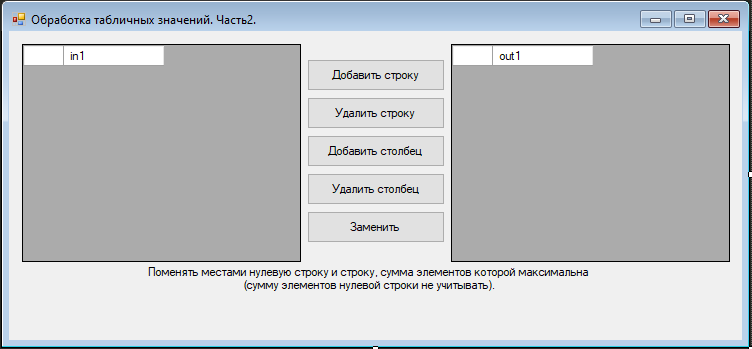
\includegraphics[width = 0.7\textwidth]{images/Task5/FormInConstructor.png}
    \caption{Вид формы в конструкторе}
    \label{fig:FormInConstruct5}
\end{figure}

\subsection{Таблица с описанием переименовнных элементов формы}

Все элементы формы были переименованы и их атрибыты изменены. Проведенные изменения представлены в таблице \ref{tab:label5}

\begin{longtable}[!h]{|l|l|l|}
    \caption{Значения атрибутов элементов в приложении <<Обработка табличных данных. Часть 2>>}
    \label{tab:label5}
    \endfirsthead
    \endhead
    \hline
    \makecell{$\textbf{Описание элементов}$\\ $\textbf{формы}$}& \makecell{$\textbf{Список измененных}$\\ $\textbf{атрибутов}$}& \makecell{$\textbf{Новое значение}$\\ $\textbf{атрибута}$}\\ 
    \hline
    \makecell{Форма}& \makecell{Text}& \makecell{Обработка табличных\\ данных 2}\\ 
    \hline
    \makecell{Первая надпись (label)}& \makecell{Name}& \makecell{taskDescription}\\ 
    \hline
    \makecell{Первая надпись (label)}& \makecell{Text}& \makecell{Поменять местами\\ нулевую строку\\ и строку,\\ сумма которой\\ максимальна (сумму\\ элементов нулевой\\ строки не учитывать)}\\ 
    \hline

    \makecell{Первая кнопка (button)}& \makecell{Name}& \makecell{btnAddRow}\\ 
    \hline
    \makecell{Первая кнопка (button)}& \makecell{Text}& \makecell{Добавить строку}\\ 
    \hline
    \makecell{Вторая кнопка (button)}& \makecell{Name}& \makecell{btnRemoveRow}\\ 
    \hline
    \makecell{Вторая кнопка (button)}& \makecell{Text}& \makecell{Удалить строку}\\ 
    \hline
    \makecell{Третья кнопка (button)}& \makecell{Name}& \makecell{btnAddColumn}\\ 
    \hline
    \makecell{Третья кнопка (button)}& \makecell{Text}& \makecell{Добавить кстолбец}\\ 
    \hline
    \makecell{Четвёртая кнопка (button)}& \makecell{Name}& \makecell{btnRemoveColumn}\\ 
    \hline
    \makecell{Четвёртая кнопка (button)}& \makecell{Text}& \makecell{Удалить столбец}\\ 
    \hline
    \makecell{Пятая кнопка (button)}& \makecell{Name}& \makecell{btnStart}\\ 
    \hline
    \makecell{Пятая кнопка (button)}& \makecell{Text}& \makecell{Заменить}\\ 
    \hline

    \makecell{Первая таблица\\ (dataGridView)}& \makecell{Name}& \makecell{dataGridInput}\\ 
    \hline
    \makecell{Вторая таблица\\ (dataGridView)}& \makecell{Name}& \makecell{dataGridOutput}\\ 
    \hline

    \makecell{Обработчик ошибок 1\\ (errorProvider)}& \makecell{Name}& \makecell{erZeroRow}\\ 
    \hline
    \makecell{Обработчик ошибок 2\\ (errorProvider)}& \makecell{Name}& \makecell{erZeroColumn}\\ 
    \hline
    \makecell{Обработчик ошибок 3\\ (errorProvider)}& \makecell{Name}& \makecell{erChanges}\\ 
    \hline
\end{longtable}

\subsection{Примеры работы}

При запуске приложения на экране появляется окно (рис.\ref{fig:StartForm5}).

\begin{figure}[!h]
    \centering
    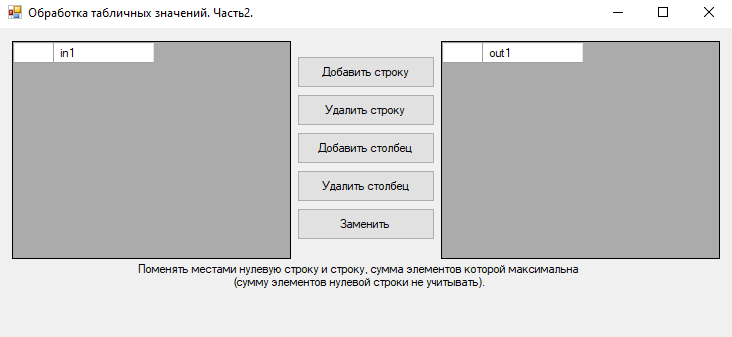
\includegraphics[width = 0.7\textwidth]{images/Task5/Start.png}
    \caption{Запуск приложения}
    \label{fig:StartForm5}
\end{figure}

При запуске с корректными данными, при нажатии на кнопку заменить происходит (рис.\ref{fig:WorkForm5}):

\newpage

\begin{figure}[!h]
    \centering
    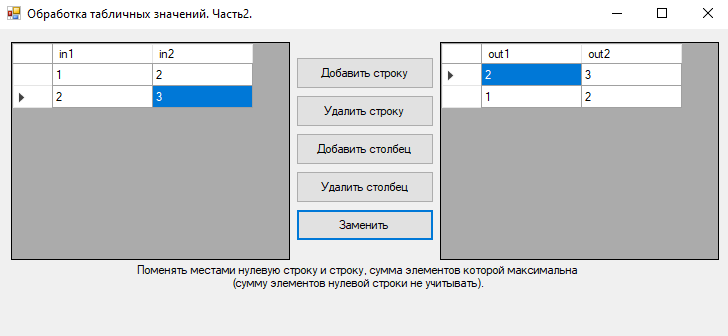
\includegraphics[width = 0.7\textwidth]{images/Task5/WorkChange1.png}
    \caption{Запуск с корректными данными}
    \label{fig:WorkForm5}
\end{figure}

При запуске с некорректными данными, при нажатии на кнопку заменить происходит  (рис.\ref{fig:BadInputNotIntForm5}):

\begin{figure}[!h]
    \centering
    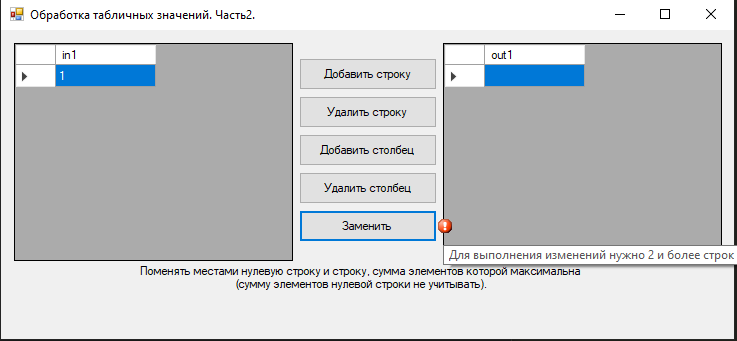
\includegraphics[width = 0.7\textwidth]{images/Task5/Try1RowChange.png}
    \caption{Запуск с некорректными данными}
    \label{fig:BadInputNotIntForm5}
\end{figure}

\subsection{Примеры кода}

Функция добавления строки в таблицу:

\begin{minted}{c++}
	// Добавление строки в таблицу
	private: System::Void btnAddRow_Click(System::Object^ sender, System::EventArgs^ e) {
		ClearAll();
		dataGridInput->Rows->Add(1);
		dataGridOutput->Rows->Add(1);
		// Увеличиваем счетчик, если добавили строку
		countRow++;
	}
\end{minted}

Функция удаления строки из таблицы:

\begin{minted}{c++}
	// Удаление строки
	private: System::Void btnRemoveRow_Click(System::Object^ sender, System::EventArgs^ e) {
		ClearAll();
		if (dataGridInput->CurrentRow == nullptr) {
			this->erZeroRow->SetError(btnRemoveRow, "Нельзя удалить не существующую строку");
			return;
		}
		if (!dataGridInput->CurrentRow->IsNewRow) {
			int input = dataGridInput->CurrentRow->Index;
			int output = dataGridOutput->CurrentRow->Index;
			dataGridInput->Rows->Remove(dataGridInput->Rows[input]);
			dataGridOutput->Rows->Remove(dataGridOutput->Rows[output]);
		}
	}
\end{minted}

Другие фрагменты кода расположены в приложении \ref{app:task5}. Полный код программы приведен в приложении \ref{app:zip}
